% ----------------------------------------
% File    : cruz_2020_05_caseStudy.tex
% Content : Multiple--Case Study section of the article for Computing
% Date    : 1/Julio/2019
% Version : 2.0
% Authors : M.Cruz 
% ----------------------------------------

% -----------------------------------
% Last update: 16/11/2020 (MCruz)
% Actualización a partir de la tesis
% -----------------------------------

%-----------------------------------------------------------
\section{Evaluation of the Template. Multiple--Case Study}
\label{sec:Case}
%-----------------------------------------------------------

Case study is a research methodology that is carried out in its natural context. Studies range from well--organised studies to small examples in a university lab \cite{runeson2009guidelines,runeson2012case}.
\emph{Multiple--case study} includes more than one case with different characteristics. If the information obtained is similar, conclusions are more solid \cite{runeson2012case}.  

We carried out a multiple--case study that includes three case studies with the main objective of evaluating the use of the template by specifying changes in the replications of selected families in three different settings.

The research method followed in this study has been based on case study research process proposed in Runeson and H{\"o}st \cite{runeson2009guidelines} and Runeson \etal \cite{runeson2012case}. 

To carry out the validation, the CÆSAR tool, developed by the authors of this paper and based on the proposed template, has been used to manage replication changes.
It has been developed using the Grails\footnote{https://grails.org/} framework on Groovy\footnote{https://groovy-lang.org/}.

The current prototype consists of three main views that allow: \emph{i)} to describe the base experiment and its replications, \emph{ii)} to specify the changes of each replication and \emph{iii)} to identify the threats to validity involved in each change.

The tool is available at https://metamodelo.herokuapp.com/. 
We are working to make the tool evolve as an assistant so that experimenters can define their replications and changes, automatically generating the \LaTeX \xspace code corresponding to the template. 

%-----------------------------------------
\subsection{Multiple--Case Study phases}
\label{sec:CS-design}
%-----------------------------------------
As shown in Fig.~\ref{fig:Multiple-CaseStudy} three main phases are identified, namely: \emph{i) Case study design}, \emph{ii) Plan, collect and analyse} and \emph{iii) Joint analysis and report}.

%------------------------------
\begin{figure}[htbp]
    \centering
    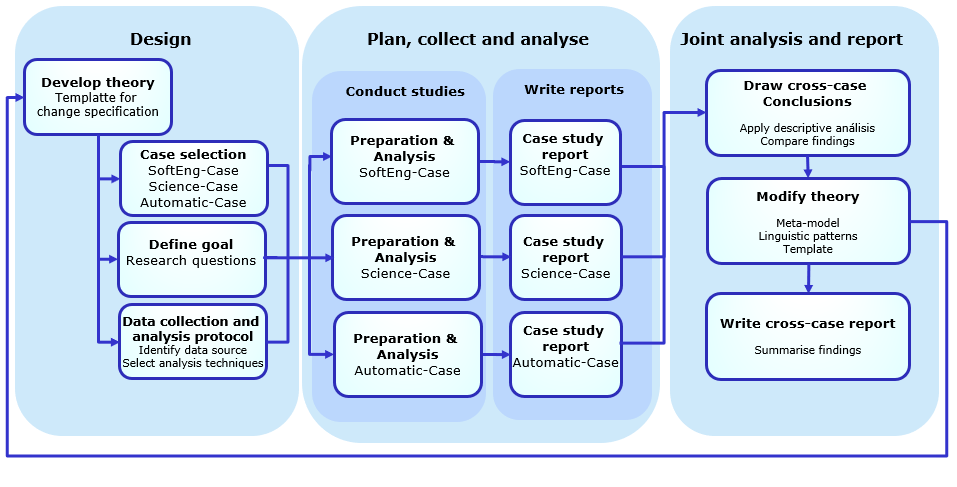
\includegraphics[width=0.9\textwidth] {figures/Multiple-Case}
     \caption{Phases of multiple--case study based on \cite{runeson2012case}}
    \label{fig:Multiple-CaseStudy} 
\end{figure}
%-------------------------------

In the first phase, \emph{case studies} have been selected and \gls{RQs} have been proposed:

%--------------------
%  Case selection
%--------------------

\begin{itemize}   
    \item \emph{Case study in Software engineering} \emph{(\SoftEng-Case)}. Initially, three families belonging to the \SE area that deal with: \emph{i) Mindfulness} (\emph{\Mind}), \emph{ii) Requirements analysis} (\emph{\Req}) and \emph{iii) Code evaluation techniques} (\emph{\Code}) were selected. 
        
    \item \emph{Case study in science} \emph{(\Science-Case)}. Afterwards, and to evaluate the usefulness of the template in other areas of knowledge, four families belonging to \emph{\Science} area and dealing with: \emph{i) Decontamination of soils} (\emph{\Soil}), \emph{ii) Quality analysis of virgin olive oil} (\emph{\Quality}), \emph{iii) Extraction  of  olive oil components} (\emph{\Olive}) and \emph{iv) Influence of diet on cholesterol accumulation} (\emph{\Diet}) were selected.
     
    \item \emph{Case study in \Automatic experiments} \emph{(\Automatic-Case)}. Finally, to evaluate the template in other types of experiments such as algorithmic experiments or those running simulations, two families of experiments on: \emph{i) Automated software testing} (\emph{\Testing}) and \emph{ii) Software Product Line testing} (\emph{\SPL}) were selected.
\end{itemize}
    

%--------------------
%  Define goal
%--------------------
In order to analyse the \emph{\expressiveness, \precision, \usability} and \emph{\traceability} of the proposed template, the following set of \gls{RQs} has been enunciated: 
   
\begin{itemize}
    \item RQ1: \emph{\Expressiveness}. What proportion of changes has it been possible to define?
    Is the \expressiveness of the template greater than other guidelines followed?

    \item RQ2: \emph{\Precision}. Through L--patterns, is the definition of changes more precise than in natural language or tables? Does it detect missing information?

    \item RQ3: \emph{\Usability}. Which fields of the template have presented understanding problems?
    Are the researchers familiar with the terminology? 
   
    \item RQ4: \emph{\Traceability}. By recording changes using the template, does it facilitate \emph{\traceability} between replications?
        
\end{itemize}
   

The second phase includes the preparation for data collection and the analysis.

%-----------------------
%  Preparation for data 
%-----------------------

According to Lethbridge et al. \cite{lethbridge2005studying} \emph{data collection techniques} can be divided into three degrees: \emph{i)} first degree of data collection techniques requires \emph{direct access} to a participant population, \emph{ii)} second degree implies \emph{access to participants environment} as they work, and \emph{iii)} third degree requires \emph{access only to work artifacts}. 
    
\begin{itemize}
    \item In \emph{\SoftEng-Case}, first family has been carried out by some of the authors of the present study. In the remaining families, the templates have also been filled by us, reading the studies that report the replications.
	
    \item In \emph{\Science-Case}, several meetings have been held with researchers belonging to the \emph{E.T.S. Ingeniería Agronómica (ETSIA)} and \emph{Instituto  de la Grasa (IG-CSIC)}. The goal of this meetings were: \emph{i)} To present and explain the use of the template; \emph{ii)} To ask each researcher to select an experiment --advised by us-- with at least one replication and, if possible, has been published; \emph{iii)} Collect the opinion of the researchers once the template has been filled in by the replication author; and \emph{iv)} Answer a questionnaire to check whether the terminology used is the same as \gls{SE}. Each template was filled in by the replication author.
    
    \item In \emph{\Automatic-Case}, researchers belonged to \gls{SE} knowledge area and they already knew the template.  The procedure was similar to the previous case. 
    Templates were filled in by us and validated by replication authors. They also answered a questionnaire about the terminology used in \emph{\Automatic experiments} and we collected their opinion.
\end{itemize}
    
\emph{Data collection techniques} from all three grades have been used:
    \emph{i)} opinions on the use and usefulness of the template have been collected through questionnaires and semi--structured interviews in the researchers' workplaces. (first and second degrees); and \emph{ii)} in order to select the families of experiments, we have used \emph{archival data}; we have reviewed the main publications of the researchers involved. \emph{Archival data} is a type of third--degree data that can be collected in a case study.   

Once the template has been completed, it is analysed whether the fields that have not been filled in are due to the different terminology used or to the lack of the required information. %
It is also analysed whether the template collects all the information that the researcher needs to reflect.
In order to fully interpret the application of the template, details such as who filled in the template (e.g. replication authors), how it was filled in (e.g. from the replication report), when it was filled in (e.g. after the replication was carried out) or whether the template was validated once filled in, are of interest.
     
\tablename~\ref{tab:compara-Case} summarizes the families of each case study along with their number of replications and changes. 
In total, the template has enabled 95 changes to be specified corresponding to 24 replications within 9 families of experiments. 
     
The complete instantiation of the replications that constitute the multiple--case study using the template, is available at the laboratory package at https://exemplar.us.es/demo/...

Table \ref{tab:template-Soil}  shows the specification of the \emph{Soil-2018} replication and its first 5 changes. \\
% ------------------------------------------------------
% File    : T-NS-Soil.tex 
% Content : Replication Soil-2018 (Carmen2018.tex)
% Date    : 2/4/2019
% Version : 1.0
% Authors : C.Florido and M.Cruz
% ------------------------------------------------------
\begin{table*}[h]
    \caption{Specification of the first 5 changes of Soil-2018 replication using the template}
  
    \label{tab:template-Soil}
    \centering
	\scriptsize

    \begin{tabularx}{\textwidth}{
        >{\hsize=0.3\hsize}X
        >{\hsize=0.7\hsize}X}
  
    \toprule

    Replication & 
    \textbf{\emph{Soil-2018}}   Internal replication based on \textbf{\emph{Soil-2016}} original experiment  \\
	
	\midrule   
     
    Description of experiment & 
        To evaluate the effect of a bio-surfactant on the assisted phytoremediation of contaminated soil \\  
 
    Site and Date & 
        The base experiment was carried out in  \textit{ETSIA-University of Seville}  in  \textit{October 2016} and this replication, in  \textit{ETSIA-University of Seville} in \textit{March 2018} \\
    
    Purpose  &  
        Generalise results \\  

\hline   
%-------------------------- 
    Change \textit{1}   & 
        \textbf{Originally}, the experiment was carried out in a cultivation chamber. \\& \textbf{In replication}, was carried out in a greenhouse \\& \textbf{In order to} simulate natural conditions \\
    
    Modified Dimension & 
        \textbf{Population}, specifically, 
        the soil type of the experimental unit soil \\
    
    Threat to validity  & 
        The change increases the external validity \\
        & since it allows to generalize the results carrying out the replication in conditions closer to natural ones \\  

\hline
%-------------------------- 
    Change \textit{2}   & 
        \textbf{Originally}, two plants were used: \emph{Hordeum vulgare} L. and \emph{Brassica juncea} L. \\& \textbf{In replication}, only \emph{Brassica juncea} L. was used \\& \textbf{Because} in the original experiment it was demonstrated that only \emph{Brassica juncea} L. was a metal accumulator plant\\  

    Modified Dimension & 
        \textbf{Protocol}, specifically experimental material \\   
        
    Threat to validity  & 
        The change does not affect validity  \\  
        
\hline
%-------------------------- 
    Change \textit{3}   & 
        \textbf{Originally}, there were two types of soil: Coria (pH=7.8) and Constantina (pH=5.5) \\& \textbf{In replication}, only Constantina soil was used \\& \textbf{Because} it was demonstrated that in the soil of Coria the metal was strongly adsorbed and the phytoextraction did not affect the biomass production   \\  
    Modified Dimension & 
        \textbf{Protocol}, specifically experimental material \\   
    
    Threat to validity  & 
        The change does not affect validity  \\  
        
\hline
%-------------------------- 
    Change \textit{4}   & 
        \textbf{Originally}, Copper (Cu) doses were 0, 500 and 1000 mg $kg^{-1}$ \\& \textbf{In replication}, Cu doses were adjusted to 0, 125, 250 and 500 mg $kg^{-1}$     \\ 
        & \textbf{Because of} Cu doses of 1000 mg $kg^{-1}$ was toxic to the plant \\  
 
    Modified Dimension & 
        \textbf{Operationalization}, specifically independent variable dosisCu \\
        
    Threat to validity & 
        The change increases internal validity because the Cu dose is adjusted to non-toxic levels for the plant \\ 

\hline
%-------------------------- 
    Change \textit{5}   & 
        \textbf{Originally}, Cu was applied as Copper Nitrate \\& \textbf{In replication}, Cu was applied as Copper Sulfate \\
        & \textbf{Because of} is more accessible and the concentrations applied do not affect the plant \\  
 
    Modified Dimension & 
        \textbf{Protocol}, specifically experimental material \\
        
    Threat to validity  & 
        The change does not affect validity  \\  
 
\bottomrule
%	\noalign{\smallskip\smallskip}\hline
	\end{tabularx}  

\end{table*}

% ------------------------------------------------------
% File    : T-Compara.tex
% Content : Compara los experimentos y replicaciones 
% Date    : 2/8/2019
% Version : 1.0
% Authors : M.Cruz
% ------------------------------------------------------
\begin{table*}[h]
    \caption{multiple--case study Summary}
    \label{tab:compara-Case}
    \centering
    \footnotesize
    \begin{tabularx}{\textwidth}{
        >{\hsize=0.4\hsize}X
        %{\hsize=0.28\hsize}X
        cccc}

	 \toprule
  
	Case study & Family & References 
	& No. replications & No. changes \\


     
	\noalign{\smallskip}\hline\noalign{\smallskip}
%    \midrule
	
 	SoftEng-Case 
 		& Mind (Mindfulness)&	
 		\cite{bernardez2014controlled,bernardez-jss-2016} 
 		& 2 & 4 \\
 		
 		& Req  (Requirements) &		
 		\cite{aranda2016estudio} 
 		& 8 & 33 \\

 		& Code (Code Evaluation) & 		\cite{juristo2003functional,juristo2012comparing,juristo2013process}
 		& 4 & 21 \\
 		
  	 	\hline
    	$\sum$ ( \textbf{SoftEng-Case}) & \textbf{3} & & \textbf{14} & \textbf{58}   \\
    	\hline
    
    Science-Case
 		& Soils (Decontamination)$^1$&	
 		\cite{madrid2016fitoextraccion,carvajal2016efecto} 
 		& 2 & 16 \\
 		
 		& Quality (Quality of Oil)$^1$&	
 		
 		& 2 & 4 \\
 		
 		& Olive  (oil components)$^2$ &		
 		\cite{garcia2016extraction}
 		& 1 & 11 \\

 		& Diet (Influence of diet)$^2$ & 					
 		\cite{pacheco2008meal} 		
 		& 1 & 1 \\
 	
	 	\hline
    	$\sum$( \textbf{Science-Case}) & \textbf{4} & &  \textbf{6} &  \textbf{32}  \\
    	\hline
    	
    Automatic-Case
 		& Testing (Testing)&	
 		\cite{parejo2016multi}
 		& 3 & 3 \\
 		
 		& SPL (Product Line)&	
 		\cite{sanchez2014comparison}
 		& 1 & 2 \\
 		
 		\hline
    	$\sum$( \textbf{Automatic-Case}) & \textbf{2} & &  \textbf{4} &  \textbf{5}  \\
    	\hline
    	
    		\hline
    	$\sum$ & \textbf{9} & &  \textbf{24} &  \textbf{95}  \\
    	%\hline
    
    
	\bottomrule
\multicolumn{3}{l}{$^1$E.T.S. Ingeniería Agronómica}  \\
%\multicolumn{3}{l}{$^2$Instituto de Recursos Naturales y Agrobiología}  \\
\multicolumn{3}{l}{$^2$Instituto  de la Grasa}  \\
	  
	\end{tabularx}  
\end{table*}
%\end{table}


In the third phase, conclusions are drawn and limitations encountered have allowed the template to evolve from its initial version.

%--------------------------------
\subsection{Multiple--case studies results}
\label{sec:CS-Results} 
%--------------------------------

\begin{itemize}
%----------------------
%  RQ1: Expressiveness
%---------------------- 
    \item[•] RQ1: \emph{\Expressiveness}. It is analyzed from two aspects:
	
	\begin{enumerate}
        \item  When defining the replications of the first \SoftEng-Case with the initial version of the template, limitations were detected due to the inability to express: 
    
        \begin{itemize}
	        \item Site and date of the baseline experiment and its replication.
	        \item Description of the experiment.
	        \item Acronym for baseline experiment and replication.
	        \item Replications on a previous replication.
	        \item \emph{Validity threats} affecting some changes.
	        \item Changes affecting context variables.
	        \item The cause of the change is unknown.
        \end{itemize}

    After the adjustments, the current version of the template has allowed to express the replications of the families belonging to the three \emph{case studies} and specifically all their changes. 

    \item On the other hand, it is of interest to analyse the \emph{\expressiveness} of the template with respect to other proposals followed by the authors of replications, such as \cite{carver2010towards,wohlin:experimentation,jedlitschka2008reporting,juristo2013basics,runeson2009guidelines}:
    
    \begin{itemize}
        
	    \item \emph{Purpose of the experiment}. In all guidelines, it is recommended to report the \emph{purpose of the experiment}. 
	
	    \item \emph{Changes to the baseline experiment and its cause}. Only in Carver's guidelines \cite{carver2010towards} --the only specific guidelines for replication-- is it recommended to report the \emph{changes} along with the causes. Similarly, Juristo and Moreno \cite{juristo2013basics} when referring to previous experiments, recommend to indicate \emph{the altered characteristics}.
	
	    \item \emph{Validity threats}. Another of the issues that should be addressed in the experiment report are the \emph{threats to validity}. It's mentioned in all the guidelines except Carver's.
	    
	    \item \emph{Use of L-pattern}. It is not used in any guide. The use of L-patters facilitates the definition of change and therefore increases \emph{\expressiveness}.

    \end{itemize}

    The proposed template include both the \emph{purpose} for carrying out the replication and the definition of the change together with the specific \emph{cause}.
    In addition, the definition of change is completed with the identification of the \emph{experimental dimension} affected and the influence of the change on the \emph{validity} of the experiment is analysed.
    
    %The full specification of the changes facilitates new replications, as corroborated by comments from experimenters in other areas involved in the \emph{multiple--case studies}.
    
    \end{enumerate}

%----------------------
%  RQ2: Precision
%---------------------- 
    \item[•] RQ2: \emph{\Precision}. Specification of changes by means of the template and L--patterns is more precise than in natural language, as it allows the lack of relevant information to be detected.
    This lack of information also includes \emph{tacit knowledge} described as knowledge that the researcher does not make explicit in the experiment report \cite{shull2002replicating}.
    
    In \SoftEng-Case, we realised that there were \emph{under-specified changes} because the \emph{cause for the change} was not specified in the report of the replication.
    Likewise, the \emph{precision} has also allowed us to realize that there are fields in the template that are difficult to complete, as confirmed by applying the template in \Science-Case, where the \emph{threats to validity} and \emph{dimension affected} by the change have only been completed in one of the four families of experiments. \\ % -- helped by us--. \newline
    
%--------------------------
%  RQ3: Usability
%--------------------------
    \item[•] RQ3: \emph{\Usability}. 
    In order to verify the \Usability of the template it is necessary that it is used by external experimenters.
    To achieve this, the \Science-case and \Automatic-case were designed with the main objective that the experimenters who have carried out the replications fill in the template. 
    
    Differences in the use of the template may be due to:

    \begin{itemize}
	    \item \SoftEng-Case. The template has been proposed in the \gls{SE} area and was filled in by us from the replication report, so logically there have been no problems of \emph{\Usability}.
	    The \emph{cause of the change} has not been fulfilled in some \emph{Req} family changes because it was not specified in the replication report.
	
	    \item \Science-Case. Experimenters have filled in the template and are unfamiliar with some of the terminology used, so it has been laborious or impossible to fill in fields such as \emph{validity threats} and \emph{dimension affected}. 
	
    	On the other hand, the rest of the template has not presented problems of \emph{\Usability}, mainly because of the help of the L--patterns that facilitate the drafting of the changes.
	
	    \item \Automatic-Case. The families in which the template has been instantiated belongs to the \gls{SE} area so the terminology is known and the template is well suited to this type of experiments.  \\

    \end{itemize}	
    
%--------------------------
%  RQ4: Traceability
%--------------------------
    \item[•] RQ4: \emph{\Traceability}. 
    The specification, using the template, of the replications that constitute the family of experiments, allows us to know the evolution of the experiment. The use of an acronym to identify replication simplifies the trace between elements.
    
    \emph{\Traceability} facilitates new replicas since by recording both the \emph{purpose of the replication} and the \emph{reason for each change}, the changes already made are known and new changes can be designed and proposed. When changes need to be made to adapt the experiment to a new environment, it may be useful to analyse the changes already made in environments with similar conditions.
     
    On the other hand, the template should be part of the \emph{laboratory package} reflecting the evolution of the experiment and establishing the trace between successive replications of the same family of experiments. \\

\end{itemize}

%----------------------------------------
% ----  Terminología      ---------------
%----------------------------------------

% -----------------------------------
% File    : T-Nomenclature.tex
% Content : Compara la nomenclatura 
% Date    : 7/Mayo/2019
% Version : 1.0
% Authors : M.Cruz
% -----------------------------------

% -----------------------------------
% Last update: 4/04/2020 (MCruz)
% Actualización a partir de la tesis
% -----------------------------------

\begin{table}
 
\caption{Comparison of nomenclature used in \SoftEng-Case, \Science-Case and \Automatic-Case}
    \label{tab:T-Nomencla}
    \centering

    \begin{tabularx}{0.95\textwidth}{Xcc}
    \toprule
   
\SoftEng-Case &  
\Science-Case & 
\Automatic-Case  \\

\noalign{\smallskip}\hline\noalign{\smallskip}
	Replication             & 
	Repetition with changes & 
	Replication             \\
	
	Repetition & 
	Repetition & 
	Repetition \\
	
	Reproduction & 
	\ding{55}    & 
	Reproduction \\
	
	Replication type & 
	\ding{55}        & 
	Replication type \\
	
	Family experiments & 
	\ding{55}          & 
	\ding{55}          \\
	
\noalign{\smallskip}\hline\noalign{\smallskip}
    Dependent variable & 
    Dependent variable & 
    Dependent variable \\
    
    Independent variable$^1$ & 
    Independent variable$^1$ &  Independent variable$^1$ \\
    
    Context variable & 
    \ding{55} & 
    Context variable \\
    
    Blocking variable &
    Blocking variable &
    Blocking variable \\
    
    Parameters & 
    Parameters & 
    Parameters \\

    Level & 
    Level &
    Level \\
  
\noalign{\smallskip}\hline\noalign{\smallskip}

    Experimental subject & 
    Experimental subject &
    \ding{55}            \\
    
    Experimental object$^2$ & 
    Experimental unit       &  
    Experimental unit       \\
    
    Population & 
    Population & 
    Population \\

\noalign{\smallskip}\hline\noalign{\smallskip}
	
    Threats to validity & 
    \ding{55}           & 
    Threats to validity \\
    
    Internal validity & 
    \ding{55}         & 
    Internal validity \\
    
    External validity & 
    \ding{55}         & 
    External validity \\
    
    Construct validity & 
    \ding{55}          & 
    Construct validity \\
    
    Conclusion validity & 
    \ding{55} & 
    Conclusion validity \\
    
\noalign{\smallskip}\hline\noalign{\smallskip}

    Experimental design & 
    Experimental design & 
    Experimental design \\
    
    Modified dimension & 
    \ding{55}          &
    \ding{55}          \\
    
    Operationalization & 
    \ding{55}          & 
    \ding{55}          \\
    
    Protocol$^3$ & 
    Procedure    & 
    Protocol     \\
    
    Treatment & 
    Treatment & 
    Treatment \\
    
    Guides & 
    Guides & 
    Guides \\

    \bottomrule
  
\multicolumn{3}{l}{$^1$ También se denomina factor}   \\ 
\multicolumn{3}{l}{$^2$ También se denomina unidad experimental  \cite{Juristo}}   \\ 
\multicolumn{3}{l}{$^3$ También se denomina procedimiento experimental}   \\
	  
\end{tabularx}  
\end{table}

Table \ref{tab:T-Nomencla} compares the terminology used in experiments in the \Science area and \Automatic experiments with the terminology used in \SE area.

Note that the term replication is not used in Science. However, it is common practice to \emph{repeat} the experiment in different seasons to confirm the results and usually some change is added (e.g. the treatment dose is adjusted). It is valuable to clearly specify such changes and their cause.

Concerning \emph{validity}, although the term \emph{validity threats} is not used, threats are considered implicitly: there is always an \emph{untreated sample} (e.g. uncontaminated control soil) and the entire design is usually repeated, increasing \emph{internal validity}.  Also, the experiments are designed, firstly, in \emph{petri dishes} or \emph{cultivation chambers} (very controlled conditions) and later in \emph{greenhouses},  gardens  or others, increasing \emph{external validity}.




